The global architecture now specified, we will introduce three related subsystems and fit them into this global framework: sensory perception --- the processing of raw sensory input into an format intelligible to other brain components ---, counterfactual perception --- the imagination, which mimics the output of the senses ---, and affect --- broadly speaking, the emotional component of cognition.

\subsection{Sensory perception}\label{sec:sensoryPerception}

The model presented herein is inspired by Marvin Minsky's ``The Emotion Machine''. Therein, Minsky proposes a layered mental structure where each successive layer operates on more and more abstract representations of the world, starting with primitive sensations and proceeding all the way to self-conscious reflection and rational planning. Figure~\ref{fig:brainLayers} shows such a layered structure.

 \begin{figure}[!h]
 	\centering
 	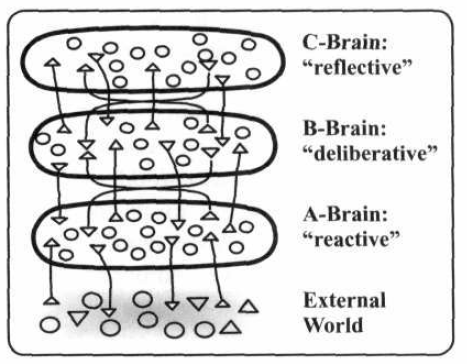
\includegraphics[width=300pt]{figs/emotionMachine_brainLayers.png}
 	\caption{Layered perception of the world, from \cite[p. 100]{emotionMachine}.}
 	\label{fig:brainLayers}
 \end{figure}
 
 \newpage
 
The diagram is explained thus \cite[p. 100]{emotionMachine}:

\begin{quote}
	Now suppose that your A-Brain gets some signals from the external world (via such organs as eyes, ears, nose, and skin) --- and that it also can react to these by sending signals that make your muscles move. By itself, the A-Brain is a separate animal that only reacts to external events but has no sense of what they might mean. For example, when the fingertips of two lovers come into intimate physical contact, {\em the resulting sensations, by themselves, have no particular implications}. For there is no significance in those signals themselves: their meanings to those lovers {\em lie in how they prepresent and process them in the higher levels of their minds.}
\end{quote}

If we apply this to the architecture of Section~\ref{fig:global}, we can devise a system in which each sense $S$ has an associated component $C_S$ which does two things:
\begin{enumerate}
	\item Consume the raw sensory information delivered by various organs and output processed input for higher brain functions;
	\item as a side a effect of this processing, cause  instinctive, low-level reactions in the body, such as pulling away from pain or jumping at a sudden fright.
\end{enumerate}

In Figure~\ref{fig:sensoryPerception}, a slice of just such a system is shown for visual, auditory, olfactory/gustatory and tactile sensation. The produced data can be of two kinds: one is more abstract than the input and facilitates deliberative action, and the other contains instructions for instinctive behaviour for the body.

\begin{figure}[!h]
	\centering
	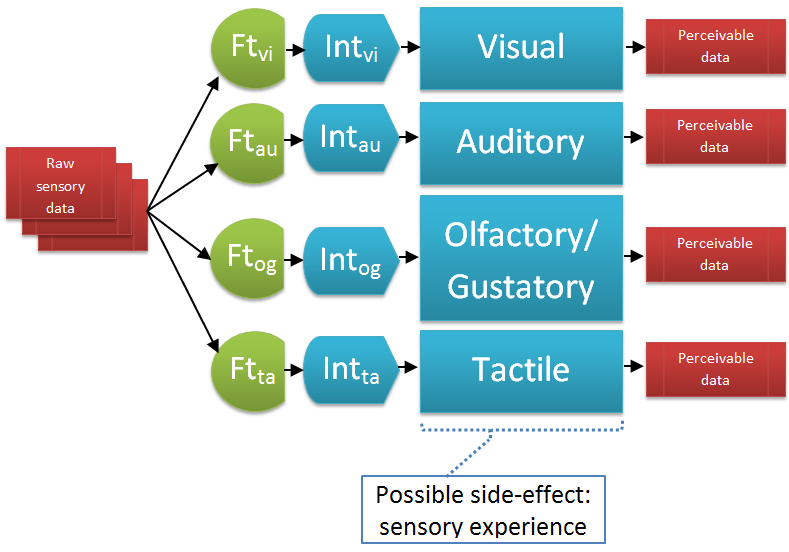
\includegraphics[width=325pt]{figs/sensoryPerception.png}
	\caption{Partial structure of sensory perception - raw sensory data is processed and made available to higher functions such as the affective subsystem. The comment ``Possible side-effect: sensory experience'' signifies the fact that conscious and sub-conscious sensory experiences might occur as a side-effect of this processing. However, it is currently unknown to neuroscience whether this is indeed the case.}
	\label{fig:sensoryPerception}
\end{figure}


\subsection{Counterfactual perception and planning}\label{sec:worldSimulation}

Broadly speaking, counterfactual perception can be described as ``imagination'', and is closely related to sensory perception and world simulation. In examining the system, we might broadly classify its processes into three categories:

\begin{enumerate}
	\item Counterfactual perception --- imagining sights, sounds, etc. Such experiences have much in common with those caused by our sensory organs, yet are marked not as real. In particular, imagined experiences evoke only parts of the conscious experience that accompanies real perceptions. Research by Berthoz and Lotze et al.\ suggests that (a) the brain indeed uses similar circuitry for real and imagined experiences and that (b) imagined experiences are prevented from being confused with real ones via inhibitory signals. Lotze et al.\ write \cite{lotze1999}:
	\begin{quote}
		The results of cortical activity support the hypothesis that motor imagery and motor performance possess similar neural substrates. The differential activation in the cerebellum during EM and IM is in accordance with the assumption that the posterior cerebellum is involved in the inhibition of movement execution during imagination.
	\end{quote}
	
	From the abstract of Berthoz's paper \cite{8713551}:
	
	\begin{quotation}
		(...) experimental evidence suggesting that the brain can use the same mechanisms for the imagination and the execution of movement. In particular the fact that adaptation of the vestibulo-ocular reflex can be obtained by pure mental effort and not solely by conflicting visual and vestibular cues has been suggestive of the fact that the brain could internally simulate conflicts and use the same adaptive mechanisms used when actual sensory cues were in conflict.
	\end{quotation}
	
	\item World simulation --- the imagination of future states. Simulating worlds goes beyond the imagination of sensory experiences; it involves constructing models of worlds and simulating their behaviour. The details of this process are unknown, but we can assert that it is capable of a number of things:
	\begin{enumerate}
		\item construction of non-physical worlds, such as mathematical models,
		\item extrapolation into the future and the past
		\item simulation of the minds itself and other agents.
	\end{enumerate}
	
	
	\item Executive planning --- humans can plan both both in immediate and concrete terms (such as body movement) and in the abstract. It is likely that different circuitry is used for movement planning and for planning involving abstract reasoning, in both cases it is necessary that the brain simulate the world in some way. The simulation of the consequences of body movement is likely older than humanity and distinct from the kind of world simulation described above, but both share their function: the agent proposes as series of actions to take, inserts them into some mental world and judges the utility of those actions based on the predicted consequences.
\end{enumerate}

Needless to say, that this process in all its subtleties is immensely complex and thus I simply endeavour to sketch its possible structure only in extremely rough outlines. This sketch is shown in Figures~\ref{fig:imagination},  \ref{fig:planner}, and \ref{fig:worldSimulatorPlannerInteraction}: the world simulation is an ordinary component with a filter and interpreter which outputs, for simplicity's sake, messages marked as counterfactual. We can imagine such messages to be very much like ordinary sensory ones, with the exceptions that they have no accompanying sensation and, more importantly, that we are aware of their non-reality. The planning component receives instructions about desirable states and outputs hypothetical actions which the world simulator incorporates. The world simulator's output is in turn read by the planner, which then abandons the plan or decides to pursue it further.

\begin{figure}
	\centering
	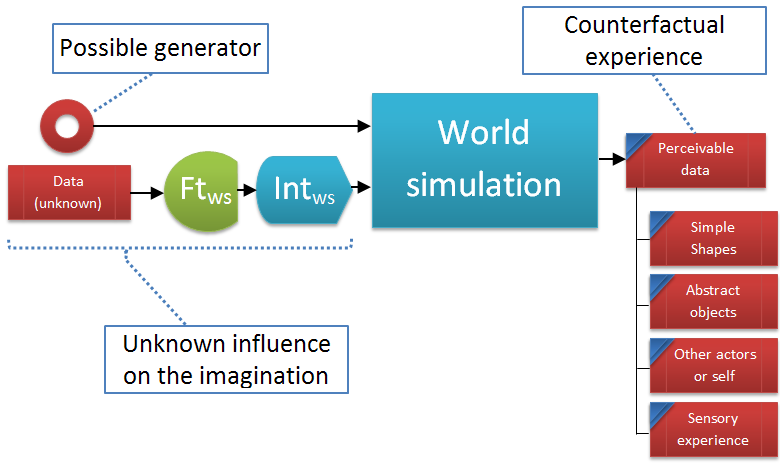
\includegraphics[width=\textwidth]{figs/imagination.png}
	\caption{Structure of of counterfactual perception \& world simulation: messages emulating the output of sensory perception are generated, but are marked as counterfactual by unknown means.}
	\label{fig:imagination}
\end{figure}

\begin{figure}
	\centering
	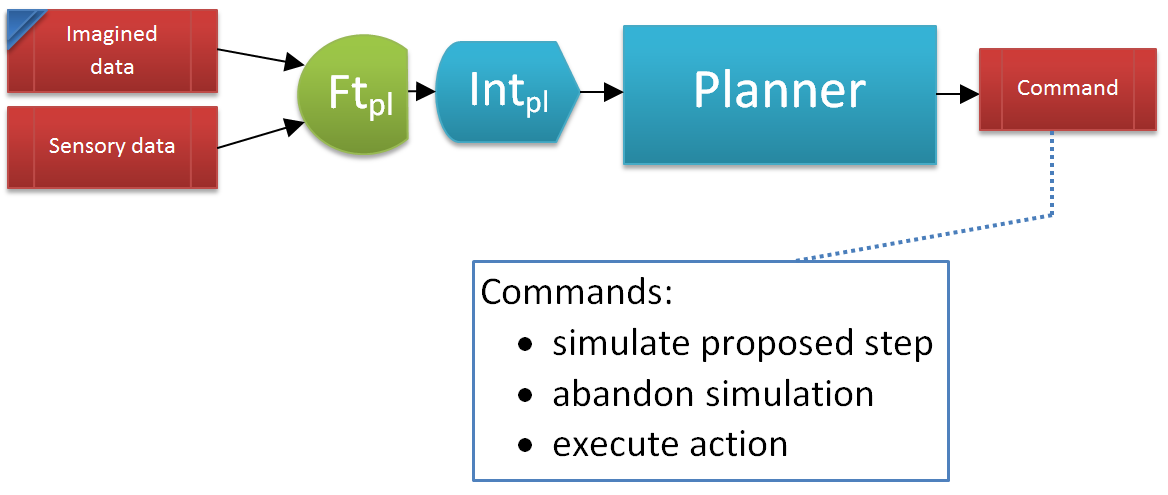
\includegraphics[width=\textwidth]{figs/planner.png}
	\caption{Planner with two kinds of inputs: (1) real sensory data and (2) counterfactual data which comes from world simulation. On the basis of these inputs, possible steps are developed and sent out as commands.}
	\label{fig:planner}
\end{figure}

The planner, minimally, has to perform two functions --- first, it has to judge the desirability of various world states and second, it has to be able to devise possible steps for the agent based on some strategy. If these two functions and some desired goal(s) are given, the planner can do its work by issuing the following commands, as shown in Figure~\ref{fig:planner}:
\begin{enumerate}
	\item If some goals are not yet reached but appear possible, devise possible steps to take and have the world simulator predict their outcomes.
	\item If the goals appear impossible the necessary steps prohibitively undesirable, command the world simulator to cease its activity.
	\item If earlier proposed steps turn out to fulfil some goal, contact the agent's executive component.
\end{enumerate}

\begin{figure}
	\centering
	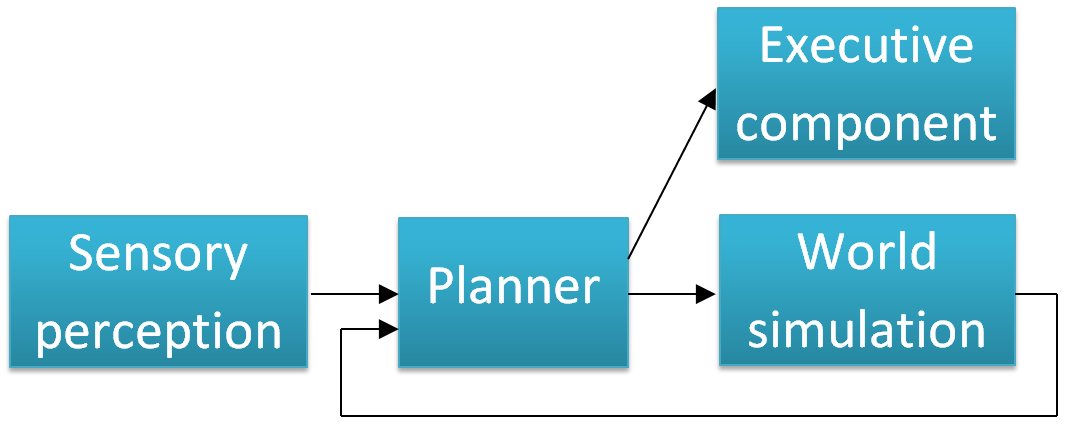
\includegraphics[width=\textwidth]{figs/worldSimulatorPlannerInteraction.png}
	\caption{Interaction between world simulator and planner: the planner devises possible steps and feeds them into the world simulator, which, in turn, tries to calculate their effects. The results are fed back to the planner.}
	\label{fig:worldSimulatorPlannerInteraction}
\end{figure}

\subsubsection{World simulation as rationality}
The way in which I just described the interaction between the world simulator and the planner suggests that they function as a pair of guesser and checker: the planner generates ideas on what to do and the world simulation tests their viability in some setting. Indeed, we can model rational thinking as embedded in the world simulator, especially if we make use of a plastic neural system. The proposed steps of the planner might be quite chaotic and irrational, but when given to the world simulator, it recognises them as such and returns a failure signal to the planner, causing it to abandon ``bad'' paths of cognition. A plastic planner can learn from the consistent failure of certain kinds of steps and, in time, propose them less and less often. Observed as a whole, this system of planner and simulator appears to simply deliver good plans by intuition, even though, in isolation, neither part is very clever.\footnote{I do not wish to idealize rationality too much; world simulation is only partly rational and, given faulty information about the world, will err considerably and in documented ways. Similarly, it is certainly possible for the planner to derange the world simulator by evaluating certain states as so desirable/undesirable that it will pursue even scenarios which the world simulator reports as highly unlikely.}

\paragraph{Model.} In a simplified way, we can model the process of logical deduction in a formal system $F = (A, R)$, where $A$ is a recursive set of axioms and $R$ is a recursive set of production rules of the form $(r_{\mt{from}}, r_{\mt{to}})$ s.t. $r_{\mt{from}} \rightarrow r_{\mt{to}}$ is a valid production in the system. Let
	\begin{enumerate}
		\item $W$ be a world simulator for the world of propositions $\mathcal{P}$ in $(A,R)$,
		\item $P$ a planner,
		\item $St = \{s_1,\dots,s_p\}$ a set of messages about steps to take,
		\item $Cat = \{K_1,\dots,K_q\}$ a list of message categories,
		\item $\tt{cur}$ the current state of the world simulator,
		\item $\tt{ins}\backslash 2$, $\tt{del}\backslash 1$ functions for inserting or deleting a state change into the world simulator or the planner,
		\item $t(i)$ and $b(i)$ functions which increase or decrease the likelihood of sending a message belonging to category $K_i$ and 
		\item $\bot_{i}, \top_{i}$ the failure and success signals of a message belonging to the category $K_i$.
	\end{enumerate}
	
One step of the interaction between $W$ and $P$, in a scenario where $P$ proposes steps $s_{i_1},\dots,s_{i_n}$, can then be modelled with two traces $T_{\mt{guess}}$ and $T_{\mt{check}}$:

$$
	\begin{array}{l l l}
		T_{\mt{guess}}(\tt{step}) & \equiv & \sendsf{P}{\tt{ins}(\tt{cur}, \tt{step})}{\tt{step}}{\tt{step}}{\tt{ins}(\tt{cur}, \tt{step})}{W}\\
		\\
		T_{\mt{check}}(\tt{step}) & \equiv &
		\forall K_i \in Cat: K_i(\tt{step}) \Rightarrow\\
		
		& & \hspace{1cm} \mt{if } \exists (cur, s_j) \in R\ \mt{ then } \
					\sendsf{W}{}{\top_i}{\top_i}{t(i)}{P}\\
		& & \hspace{1cm} \mt{else }\ \sendsf{W}{\tt{del}(\tt{step})}{\bot_i}{\bot_i}{\tt{del}(\tt{step}), b(i)}{P}\\
	\end{array}
$$

\medskip

Axioms can be selected by executing $T_{\mt{guess}}(\tt{ax})$ for all $\tt{ax} \in A$. We can then perform deduction via $T_{\mt{guess}};T_{\mt{check}}$, for a probabilistically selected $\tt{step} \in St$.

Intuitively, $T_{\mt{guess}}$ guesses a step to take. It does so but inserting it into the planner's world-state via $\tt{ins}$ and then sending a message to the world simulator, which also inserts it into its world state. $T_{\mt{check}}$ then checks whether the change from $\tt{cur}$ to $\tt{step}$ was legitimate. If so, it determines to which category $\tt{step}$ belongs and sends the $\top$-signal for that category back to the planner. Otherwise, it sends the corresponding $\bot$-signal. The purpose of this is to make it more or less likely, respectively, that the planner should choose the same category of step in the future. The categories, we can imagine, could be things like ``modus ponens'', ``associative reasoning'', ``appeal to consequences'' and so forth.

If we repeat this interaction (with different proposed steps $s_1,\dots,s_p$ in each iteration), we get an algorithm for logical deduction  --- that is, since $A$ and $R$ are recursive, the system will recursively enumerate all valid logical formulas, provided that we pursue each path and that the probability of selecting any valid step is $> 0$. In addition, we could add a goal function $g$ to $P$ s.t. it would accept certain states and stop. Thereby, $P$ and $W$ could be used to prove logical propositions.

\subsection{Affect}\label{sec:affect}

When discussing human affect, one can mean various things: the causation of emotion, its internal mechanisms, the expression of emotion, social communication of emotions, etc. In this document, we restrict our attention just to the internal mechanisms --- that is, to the means by which emotions are evoked in an agent and how they shape its thinking.

Furthermore, the issue will only be the causative mechanism itself; taxonomy and hierarchy of emotions are deferred to future versions of this document.

The model presented herein is adapted from Gadanho and Hallam \cite{DBLP:journals/adb/GadanhoH01}, who employed it in the context of robot learning. They constructed a system of \caps{feelings} and \caps{sensations} $\mathcal{F}$, \caps{emotions} $\mathcal{E}$, and a hormone storage $H$.

\begin{figure}[!h]
	\centering
	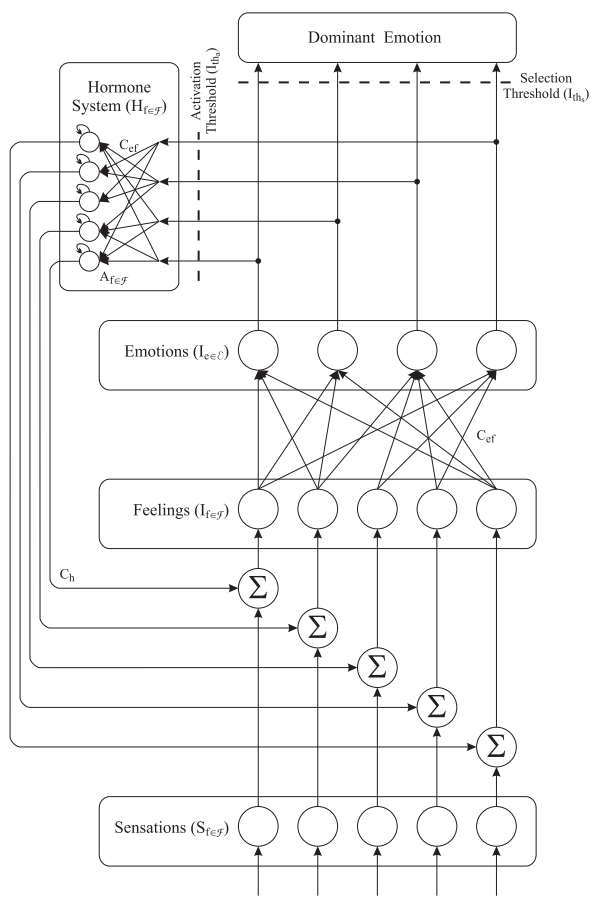
\includegraphics[width=200pt]{figs/gadanhoModel.png}
	\caption{Emotional model of Gadanho and Hallam \cite[p. 46]{DBLP:journals/adb/GadanhoH01}.}
	\label{fig:gadanhoModel}
\end{figure}

Figure~\ref{fig:gadanhoModel} shows this model: \caps{sensations} enter the system and are connected to the \caps{feelings}. They, in turn, determine the agent's \caps{emotions}. The emotions then feed into a \caps{hormone storage}, the contents of which influence, together with the \caps{sensations}, the agent's \caps{feelings}. In the context of their paper, this model had a very restricted application. Its purpose was to merely help guide a robot through a world, and accordingly, $\mathcal{F}$ and $\mathcal{E}$ were only defined as \cite[p. 47]{DBLP:journals/adb/GadanhoH01}:
$$
	\begin{array}{l}
		\mathcal{F} = \{ \mt{Hunger}, \mt{Pain}, \mt{Restlessness},
						 \mt{Temperature}, \mt{Eating}, \mt{Smell},
						 \mt{Eating}, \mt{Proximity} \}\\
		\mathcal{E} = \{ \mt{Happiness}, \mt{Sadness}, \mt{Fear},
						 \mt{Anger} \}
	\end{array}
$$

\begin{figure}[!h]
	\centering
	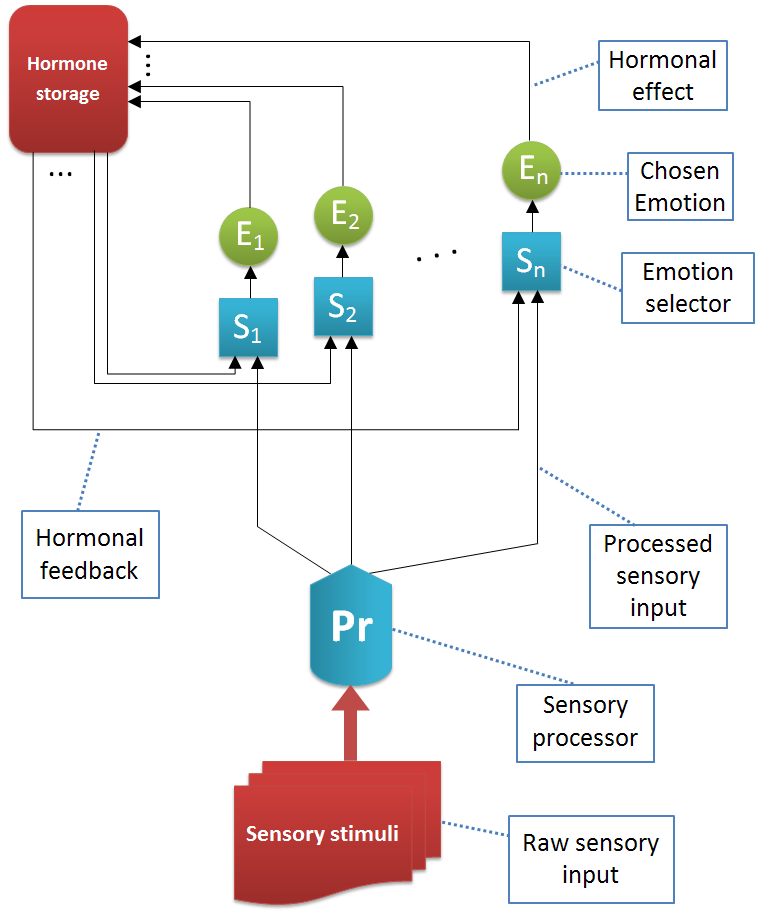
\includegraphics[width=400pt]{figs/affectiveSubsystem.png}
	\caption{Affective subsystem; specialisation of the global neural architecture. In plastic neural systems, selections may change over time.}
	\label{fig:affectiveSubsystem}
\end{figure}

\pagebreak
The main advantage of Gadanho's and Hallam's model is that (a) it is sufficiently generic to accommodate various schemas and (b) posits an internal state (the hormone storage), giving agents a certain inertia. For example, one can imagine integrating a many-dimensional model like Brazeal's \cite{breazeal2003} detailed taxonomy of emotion like Ortony's OCC model \cite{ortony1988}. The existence of an internal state is necessitated by the simple observation that our internal world is not solely dependent on momentary stimuli, but merely influenced by them. The idea of a hormone storage might be a simplistic approximation but it, too, can be refined as needed.\footnote{It might be tempting to simply replace the hormone storage with the message space, but doing so would ignore the role that neurotransmitters like dopamine and serotonin play in cognition, irrespective of the purely computational activity of brain components.} Figure~\ref{fig:sensoryPerception} shows the adapted model. The general structure was retained, but the set of sensations was replaced by the sensory processor described in Section~\ref{sec:sensoryPerception} and, instead of a single dominant emotion, competing emotions simply emit messages which are used by execute components and the world simulation.

\subsubsection{Affective subsystems}

In this section, I will develop the concept of ``emotion'' in greater detail. The process shown in Figure~\ref{fig:affectiveSubsystem} might suggest we simply have a collection of emotions and that all emotions are essentially equal, but I submit that this is not so. Instead, I propose the existence of various subsystems, each responsible for a group of emotions, and each with its own history and distinctive tasks. In the rest of this work, the following two assumptions will be made:

\begin{enumerate}
	\item {\em ``Emotion'' is not a singular phenomenon.} Specifically, this is contradicts many-dimensional models of emotions which propose one, two, three or four axes and a corresponding vector space in which every emotion is a point. Such a view implies that all emotions share a neurological template which is parametrized with coordinates to result in different experiences.
	\item {\em There exist emotions which are both different in kind and which pertain to different subsystems in the brain.} This implies that emotions cannot morally be seen as a homogeneous set $\{E_1,\dots,E_n\}$. Instead, a number of distinct subsystems are necessitated, each responsible for the causation and processing of a group of emotions. Given this, the only substantial aspect any two emotions might have in common would be our referring to both of them as ``emotion''.
\end{enumerate}

Both of these assumptions are rather concrete and thus deserve evidence. In 1999, Davidson and Irwin, using PET and fMRI scanning, found two different systems mediating approach- and avoidance related behaviors \cite[p. 13]{davidson1999}:

\begin{quote}
A large body of lesion, neuroimaging and electrophysiological data supports the view that the prefrontal cortex (PFC) is an important part of the circuitry that implements both positive and negative affect. ($\dots$)
A number of early studies that evaluated mood subsquent to brain damage suggested that patients with damage to the left hemisphere, particularly in PFC, were more likely to develop deppressive symptoms compared with patients having lesions in homologous regions of the right hemisphere. ($\dots$)
The general finding of left dorso-lateral PFC damage increasing the likelihood of deppressive symptoms has been interpreted to reflect the contribution of this cortical territory to certain features of positive affect, which, when disrupted, increases the probability of depressive symptomatology.
\end{quote}

In this, they echo earlies findings by Cacioppo et al.\ \cite{cacioppo1999}, Gray \cite{gray1994} and Lang et al.\ \cite{lang1990} that affect is lateralized, with different hemispheres being responsible for different categories of feeling. It therefore stands to reason that different emotions, being generated by different brain regions, should therefore also be different in their character.

Further, much research has been done in the area of so-called {\em basic emotions} --- a small set of emotions are acknowledged as being both elementary and characteristically distinct from each other. The Cambridge Handbook of Affective Neuroscience provides a good overview of the basic emotion theory \cite[pp. 9-10]{cambridgeAff}. Matsumoto and Eckman \cite{matsumoto2009}, for instance, identified seven basic emotions: happiness, surprise, contempt, sadness, fear, disgust, and anger.

Damasio \cite{damasio1998}, drawing upon neuroscientific findings, sketches a model of affect mainly involving the prefrontal cortex, but also the amygdala, the hypothalamus, and the anterior cingulate cortex, as seen in Figure~\ref{fig:damasioSystem}.

\begin{figure}
	\centering
	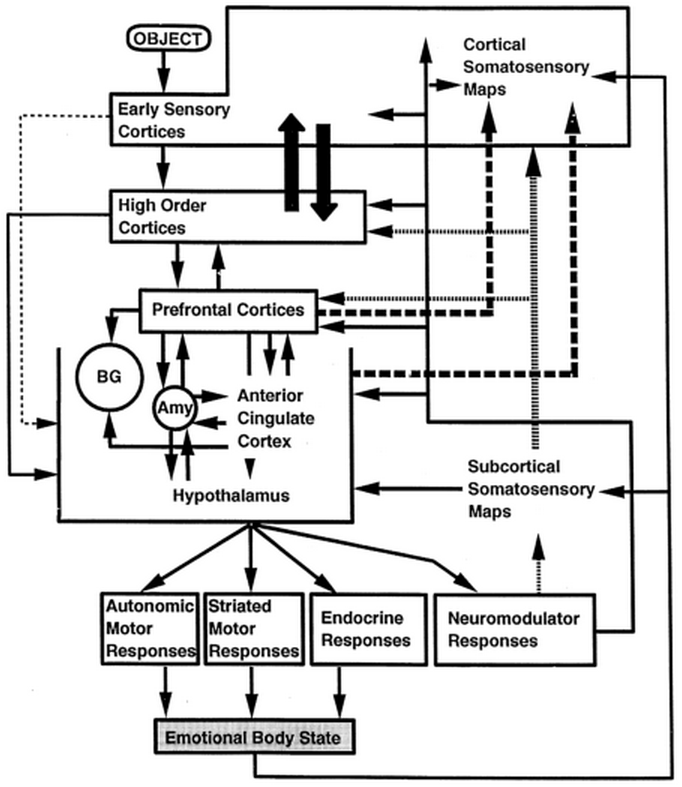
\includegraphics[width=250pt]{figs/damasioSystem.png}
	\caption{Neurological structure of affect, according to Damasio \cite{damasio1998}.}
	\label{fig:damasioSystem}
\end{figure}

In the same article, he describes how different brain regions are responsible for different kinds of emotion:

\begin{quotation}
	Equally problematic is the widespread view that the limbic system is the neural basis for all emotions. A rich body of evidence tells us that this is just not the case. Both within and around the limbic system, circuitry connection varied neural sites supports the operation of different emotion. For instance, work on aversive conditioning in rodents has shown that the amygdala is certainly involved in negative emotions such as fear [10,6]. {\em Work in humans, on the other hand, has not only confirmed the amygdala's involvement in negative emotions such as fear and anger, but also shown that the amygdala is not involved in the processing of positive emotions such as happiness, or negative emotions such as disgust.} [emphasis mine]
\end{quotation}

The last sentence of that quotation is especially revealing: it states that the neurological distinction is not simply one between positive and negative, or one between approach- or avoidance-related emotions, but that each emotion has its own profile of neurological activity and involves its own peculiar set of brain structures.

These facts make it quite clear that emotions are not simply homogeneous phenomena, being induced by a single system in the brain; rather, they are different in character and in the neural structures they involve. 

\paragraph{Structure of affect} The system depicted in Figure~\ref{fig:affectiveSubsystem} left several parts unspecified: the sensory processor $\Pr$, the emotion selectors $S_1,\dots,S_n$ and the messages sent by the chosen emotions into the message space. In the following paragraphs, I will flesh out that model in greater detail, building principally on the work of Sander, Grandjean and Scherer \cite{DBLP:journals/nn/SanderGS05}. Sander and colleagues partitioned the emotion process into four stages, as shown in Figure~\ref{fig:sanderSystem}. The first is {\em relevance}, which functions as a filter and detects the intrinsic pleasantness and the level of (emotional) attention that a stimulus demands. The processes of this stage, roughly speaking, correspond to the work of the sensory processor $\Pr$. The second stage is {\em implication}, where reasoning becomes engaged in order to determine the cause, likely outcome, and urgency of the perceived facts. At this stage, emotions like joy, anger, contentment, disgust, etc. are evoked, together with approach- and avoidance-related behaviours --- this corresponds to the emotion selectors $S_1,\dots,S_n$. Deliberate strategies come only in the next stage: {\em coping}. In it, reasoning and planning become fully engaged. The fourth stage is {\em normative significance} and deals, in essence, with moral concerns, both internal and those of other agents.

\begin{figure}
	\centering
	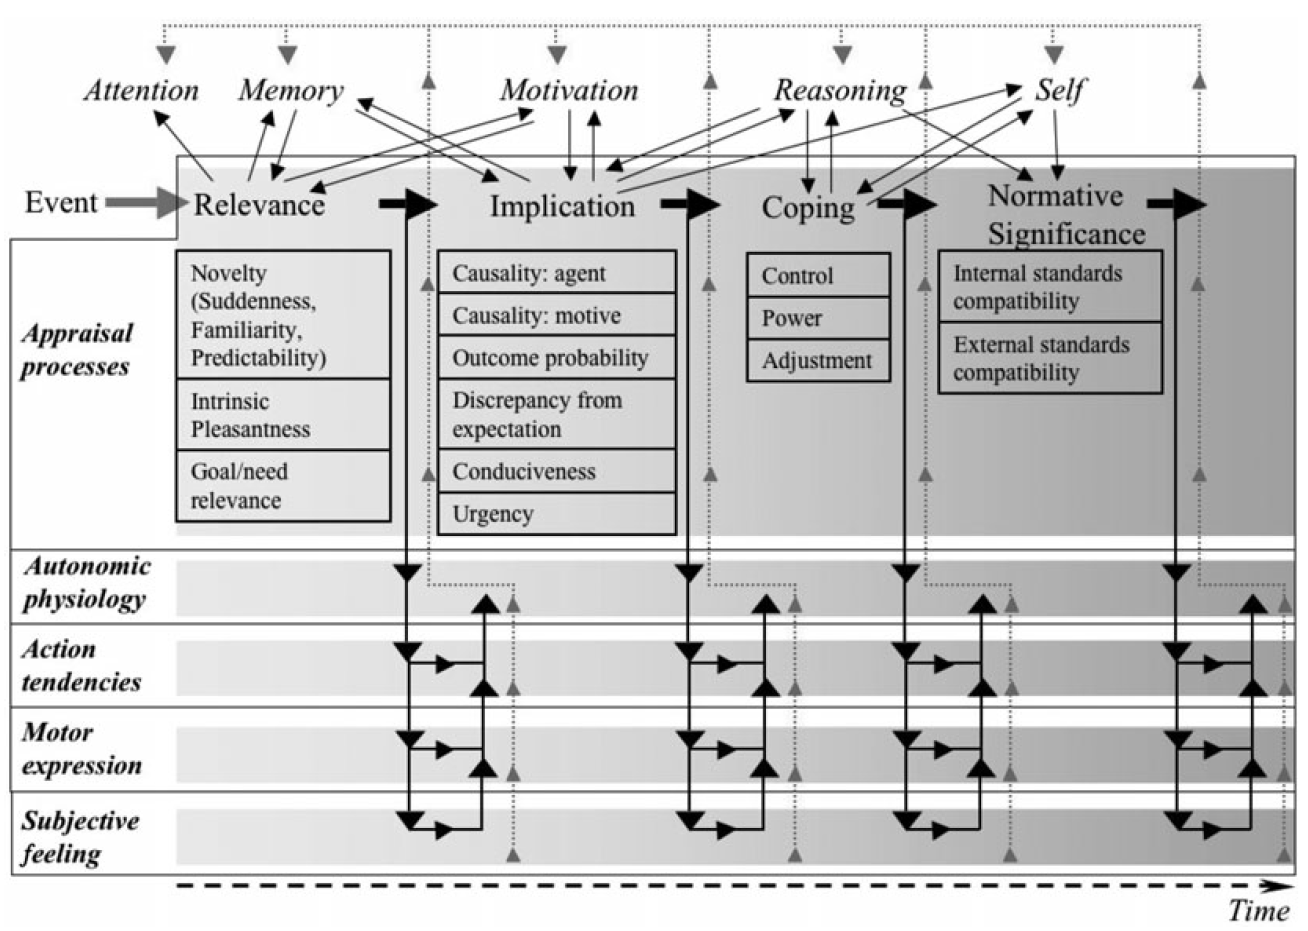
\includegraphics[width=440pt]{figs/sanderSystem.png}
	\caption{The four-stage emotion process according to Sander et al, consisting of relevance, implication, coping and normative significance.}
	\label{fig:sanderSystem}
\end{figure}

Sander et al.\ give a good, detailed account of the interactions of affect with other systems, although I would argue that theirs is unduly suggestive of a simple {\em pipeline}., rather than a mesh of systems into which the affective ones are embedded. In addition, it does not address the interactions with perception, memory, and reasoning. Based on the evidence discussed above, I shall now present a more horizontal view and construct a model of the hypothesized emotional subsystems and their interactions with other parts of the brain. Since no established vocabulary seems to exist in this specific are I shall first introduce a number of terms.

\begin{definition}[Evocative system]
An evocative system is a subsystem in the brain responsible for evoking consciously experienced affect within an agent based on internal or external stimuli.
\end{definition} 

Various such evocative systems can be imagined. I propose the following rough categorization:

\begin{description}
	\item[Pre-social emotions.] Certain behavioural mechanisms can be observed in non-social as well as social animals. The flight-or-flight instinct, for example, is nearly universal, as is the inclination to seek out food, shelter, and other resources. ``Instinct'' is indeed a more appropriate term in the case of most species, rather than ``emotion'', which connotes a certain richness of experience. Nonetheless, we can clearly see that, in more intelligent, social animals, emotions like anger, fear, and joy, have grown out of just these instincts. Hence the term ``pre-social emotions'': while emotion itself is quite possibly inherently social, certain emotions are rooted in instincts which are not, and an emotional animal would feel them even if it were the only one of its kind in an environment.
	
	\item[Social emotions.] A by far richer subset of emotions are the social ones. Indeed, social situations are the ones where affect can and must truly shine: the presence of other individuals the entire tribe demand a variety of affect relating to the appraisal of the agents, sympathy/antipathy, respect/contempt, the appraisal of oneself, showing dominance or submission, influencing other group members, taking action as a group, judging the behaviour of agents against norms, etc. It is also in social emotions in which it even makes sense to {\em show} emotion: facial expressions and gestures provide the signalling and mechanism needed for group coherence and coordinated action.
	
	We can identify several subsystems in the category of social emotion:
	
	\begin{enumerate}
		\item Reflective judgement about oneself in relation to the group or to abstract norms, primarily pride and shame \cite{Teroni2008}, but possibly also jealousy and humiliation (which, in contrast to shame, is attributed to external causes) \cite{fontaine2009};
		\item other-related judgement which determines whether to feel sympathy or antipathy, compassion, respect or contempt, trust or distrust for other individuals;
		\item normative judgement, which determines whether others or oneself is acting in accordance with instinctive or cultural norms.
	\end{enumerate}
	
	Other classifications are also possible. Haidt \cite{haidt2003}, for example, identifies those that are other-condemning (disgust, contempt), self-conscious (shame, embarrassment), other-suffering (compassion), other-praising (gratitude, awe). The picture is immensely complex and the neurological structure is presently not known. For the purposes of this thesis, we will therefore content ourselves with only this roughest of outlines.
	
	\item[Aesthetic emotions.] This type of emotion is perhaps the least studied in neuroscience and AI. It is certainly the most subtle and the least ``utilitarian'' type --- as such, it is philosophers, rather than AI researchers, who study it. For instance, Jenefer Robinson, in {\em Deeper Than Reason: Emotion and Its Role in Literature, Music, and Art} \cite{robinson2005}, writes about the affective appraisal of artwork as an unconscious process which partly reproduces the emotions of its creator. In this, she builds upon and modifies Collingwood's 1983 {\em The Principles of Art} \cite{collingwood1938, SEPcollingwood}. Since aesthetics are not the focus of this work, I shall leave it at this mention. A more thorough exploration would be interesting future work, however.
\end{description}

The emotions just listed can all be found in the more extensive taxonomies, chiefly among them in Ortony's OCC model \cite{ortony1988}. The taxonomies, however, tend to neglect the underlying neurology and the chronology of the development of these systems. Ortony's classification specifically is persuasive up to a point, but, despite it being fine-grained, one is left wondering about the underlying structure: which emotions are caused by the same brain regions, what structure, if any, do two given emotions share, to what degree is the classification scheme isomorphic to the actual neurology? This is an active area of research and while these questions are interesting, we have to leave them largely open for now.

Evocative systems tie into and directly influence

\begin{definition}[Executive system]
An executive system is a subsystem in the brain which regulates attention, makes decisions, and causes deliberate motor action in an agent.
\end{definition}

Up to this point, the executive functions have not been discussed in detail, as they are not the focus of this work. Any description of affect, however, would be incomplete without them, as attentional and behavioural changes are the sole point of emotions. Very broadly speaking, we can divide executive functions into four categories:

\begin{enumerate}
	\item \textbf{sub-conscious motor control}: instinctive reaction, such as the jerking away from pain, jumping when startled, and turning towards interesting visual stimuli;
	\item \textbf{conscious motor control}: deliberate, planned action which the agent experiences as a choice;
	\item \textbf{sub-conscious mental control}: involuntary but consciously experienced changes to the mind-state of an agent which are perceived as activity rather than mere feeling. This includes like obsessing over an issue, manias, fantasies insofar as involuntary, etc.
	\item \textbf{conscious mental control}: deliberate mental changes of an agent. This includes the making of decisions, the deliberate focusing of attention, deliberate planning, deliberate strategy selection, and so forth.
\end{enumerate}

\paragraph{Pre-social behavior control} 

\paragraph{Social judgement system}

\paragraph{Social reflective system}

\paragraph{Aesthetic judgement system}